% !TeX spellcheck = en_GB
% !TeX encoding = UTF-8
\documentclass[10pt, a4paper, landscape]{article}

% ----- packages -----
\usepackage{amsmath} % AMS mathematical facilities for LaTeX
\usepackage{amssymb}
\usepackage{enumitem} % Control layout of itemize, enumerate, description
\usepackage{fancyhdr} % Extensive control of page headers and footers in LaTeX2
\usepackage{geometry} % Flexible and complete interface to document dimensions
\usepackage{graphicx} % Enhanced support for graphics
\usepackage{hyperref} % Extensive support for hypertext in LaTeX
\usepackage{multicol} % Intermix single and multiple columns
\usepackage{parskip} % Layout with zero \parindent, non-zero \parskip
\usepackage{tikz} % Create PostScript and PDF graphics in TeX
\usepackage{titlesec} % Select alternative section titles

% ----- pdf metadata -----
\hypersetup{
	pdftitle={Additional Cheat Sheet},
	pdfsubject={The Econometrics Cheat Sheet Project - marcelomijas - CC-BY-4.0},
	pdfauthor={Marcelo Moreno Porras},
	pdfkeywords={statistics, latex, economics, cheatsheet, econometrcis, ols-regression, economic-modelling},
	pdfduplex={DuplexFlipShortEdge}
}

% ----- random seed -----
\pgfmathsetseed{10}

% ----- custom commands -----
\DeclareMathOperator{\E}{E}
\DeclareMathOperator{\Var}{Var}
\DeclareMathOperator{\se}{se}
\DeclareMathOperator{\Cov}{Cov}
\DeclareMathOperator{\Corr}{Corr}
\DeclareMathOperator{\rk}{rk}
\DeclareMathOperator{\Cr}{Cr}
\DeclareMathOperator{\AIC}{AIC}
\DeclareMathOperator{\HQ}{HQ}
\DeclareMathOperator{\BIC}{BIC}
\newcommand{\SSR}{\text{SSR}}
\newcommand{\SSE}{\text{SSE}}
\newcommand{\SST}{\text{SST}}
\newcommand{\trend}{\text{Trend}_{t}}
\newcommand{\const}{\text{const}}

% ----- page customization -----
\geometry{margin=1cm} % margins config
\pagenumbering{gobble} % remove page numeration
\setlength{\parskip}{0cm} % paragraph spacing
% title spacing
\titlespacing{\section}{0pt}{2ex}{1ex}
\titlespacing{\subsection}{0pt}{1ex}{0ex}
\titlespacing{\subsubsection}{0pt}{0.5ex}{0ex}

% ----- footer -----
\pagestyle{fancy}
\renewcommand{\headrulewidth}{0pt}
\cfoot{\href{https://github.com/marcelomijas/econometrics-cheatsheet}{\normalfont \footnotesize ADD-25.08.1-EN - github.com/marcelomijas/econometrics-cheatsheet - CC-BY-4.0 license}}
\setlength{\footskip}{12pt}

% ----- document -----
\begin{document}

\begin{multicols}{3}

\begin{center}
	\textbf{\LARGE \href{https://github.com/marcelomijas/econometrics-cheatsheet}{Additional Cheat Sheet}}

	{\footnotesize By Marcelo Moreno Porras - Universidad Rey Juan Carlos}

	{\footnotesize The Econometrics Cheat Sheet Project}
\end{center}

\section*{OLS matrix notation}

The general econometric model:

\begin{center}
	\( y_{i} = \beta_{0} + \beta_{1} x_{1i} + \cdots + \beta_{k} x_{ki} + u_{i} \)
\end{center}

Can be written in matrix notation as:

\begin{center}
	\( y = X \beta + u \)
\end{center}

Let's call \( \hat{u} \) the vector of estimated residuals \( (\hat{u} \neq u) \):

\begin{center}
	\( \hat{u} = y - X \hat{\beta} \)
\end{center}

The \textbf{objective} of OLS is to \textbf{minimise} the \( \SSR \):

\begin{center}
	\( \min \SSR = \min \sum_{i = 1}^{n} \hat{u}_{i}^{2} = \min \hat{u}^{\top} \hat{u} \)
\end{center}

\begin{itemize}[leftmargin=*]
	\item Defining \( \hat{u}^{\top} \hat{u} \):
	\begin{center}
		\( \hat{u}^{\top} \hat{u} = (y - X \hat{\beta})^{\top} (y - X \hat{\beta}) \)

		\( = y^{\top} y - 2 \hat{\beta}^{\top} X^{\top} y + \hat{\beta}^{\top} X^{\top} X \hat{\beta} \)
	\end{center}
	\item Minimizing \( \hat{u}^{\top} \hat{u} \):
	\begin{center}
		\( \frac{\partial \hat{u}^{\top} \hat{u}}{\partial \hat{\beta}} = -2 X^{\top} y + 2 X^{\top} X \hat{\beta} = 0 \)

		\( \hat{\beta} = (X^{\top} X)^{-1} (X^{\top} y) \)

		\scalebox{0.85}{
			\(
			\begin{bmatrix}
				\beta_{0} \\
				\beta_{1} \\
				\vdots    \\
				\beta_{k}
			\end{bmatrix}
			=
			\begin{bmatrix}
				n          & \sum x_{1}       & \hdots & \sum x_{k}       \\
				\sum x_{1} & \sum x_{1}^{2}   & \hdots & \sum x_{1} x_{k} \\
				\vdots     & \vdots           & \ddots & \vdots           \\
				\sum x_{k} & \sum x_{k} x_{1} & \hdots & \sum x_{k}^{2}
			\end{bmatrix}^{-1}\cdot
			\begin{bmatrix}
				\sum y       \\
				\sum y x_{1} \\
				\vdots       \\
				\sum y x_{k}
			\end{bmatrix}
			\)
		}
	\end{center}
	The second derivative \( \frac{\partial^{2} \hat{u}^{\top} \hat{u}}{\partial \hat{\beta}^{2}} = X^{\top} X > 0 \) (is a min.)
\end{itemize}

\section*{Variance-covariance matrix of \( \hat{\beta} \)}

Has the following shape:

\begin{center}
	\( \Var(\hat{\beta}) = \hat{\sigma}_{u}^{2} \cdot (X^{\top} X)^{-1} \)
\end{center}

\begin{center}
	\scalebox{0.85}{ 
		\( =
		\begin{bmatrix}
			\Var(\hat{\beta}_{0})                  & \Cov(\hat{\beta}_{0}, \hat{\beta}_{1}) & \hdots & \Cov(\hat{\beta}_{0}, \hat{\beta}_{k}) \\
			\Cov(\hat{\beta}_{1}, \hat{\beta}_{0}) & \Var(\hat{\beta}_{1})                  & \hdots & \Cov(\hat{\beta}_{1}, \hat{\beta}_{k}) \\
			\vdots                                 & \vdots                                 & \ddots & \vdots                                 \\
			\Cov(\hat{\beta}_{k}, \hat{\beta}_{0}) & \Cov(\hat{\beta}_{k}, \hat{\beta}_{1}) & \hdots & \Var(\hat{\beta}_{k})
		\end{bmatrix}
		\)
	}
\end{center}

\quad where: \( \hat{\sigma}_{u}^{2} = \frac{\hat{u}^{\top} \hat{u}}{n - k - 1} \)

The standard errors are on the diagonal of:

\begin{center}
	\( \se(\hat{\beta}) = \sqrt{\Var(\hat{\beta})} \)
\end{center}

\section*{Error measurements}

\begin{itemize}[leftmargin=*]
	\item \( \SSR = \hat{u}^{\top} \hat{u}= y^{\top} y - \hat{\beta}^{\top} X^{\top} y = \sum(y_{i} - \hat{y}_{i})^{2} \)
	\item \( \SSE = \hat{\beta}^{\top} X^{\top} y - n \overline{y}^{2} = \sum(\hat{y}_{i} - \overline{y})^{2} \)
	\item \( \SST = \SSR + \SSE = y^{\top} y - n \overline{y}^{2} = \sum(y_{i} - \overline{y})^{2} \)
\end{itemize}

\columnbreak

\section*{Variance-covariance matrix of \( u \)}

Has the following shape:

\begin{center}
	\( \Var(u) = \)
	\scalebox{0.85}{
		\(
		\begin{bmatrix}
			\Var(u_{1})        & \Cov(u_{1}, u_{2}) & \hdots & \Cov(u_{1}, u_{n}) \\
			\Cov(u_{2}, u_{1}) & \Var(u_{2})        & \hdots & \Cov(u_{2}, u_{n}) \\
			\vdots             & \vdots             & \ddots & \vdots             \\
			\Cov(u_{n}, u_{1}) & \Cov(u_{n}, u_{2}) & \hdots & \Var(u_{n})
		\end{bmatrix}
		\)
	}
\end{center}

Under no heteroscedasticity and no autocorrelation, the variance-covariance matrix:

\begin{center}
	\( \Var(u) = \sigma_{u}^{2} \cdot I_{n} = \)
	\scalebox{0.85}{
		\(
		\begin{bmatrix}
			\sigma_{u}^{2} & 0              & \hdots & 0              \\
			0              & \sigma_{u}^{2} & \hdots & 0              \\
			\vdots         & \vdots         & \ddots & \vdots         \\
			0              & 0              & \hdots & \sigma_{u}^{2}
		\end{bmatrix}
		\)
	}
\end{center}

\quad where \( I_{n} \) is an identity matrix of \( n \times n \) elements.

Under \textcolor{cyan}{\textbf{heteroscedasticity}} and \textcolor{magenta}{\textbf{autocorrelation}}, the variance-covariance matrix:

\begin{center}
	\( \Var(u) = \sigma_{u}^{2} \cdot \Omega = \)
	\scalebox{0.85}{
		\(
		\begin{bmatrix}
			\textcolor{cyan}{\sigma_{u_{1}}^2}   & \textcolor{magenta}{\sigma_{u_{12}}} & \hdots & \textcolor{magenta}{\sigma_{u_{1n}}} \\
			\textcolor{magenta}{\sigma_{u_{21}}} & \textcolor{cyan}{\sigma_{u_{2}}^2}   & \hdots & \textcolor{magenta}{\sigma_{u_{2n}}} \\
			\vdots                               & \vdots                               & \ddots & \vdots                               \\
			\textcolor{magenta}{\sigma_{u_{n1}}} & \textcolor{magenta}{\sigma_{u_{n2}}} & \hdots & \textcolor{cyan}{\sigma_{u_{n}}^2}
		\end{bmatrix}
		\)
	}
\end{center}

\quad where \( \Omega \neq I_{n} \).

\begin{itemize}[leftmargin=*]
	\item Heteroscedasticity: \( \Var(u) = \sigma_{u_{i}}^{2} \neq \sigma_{u}^{2} \)
	\item Autocorrelation: \( \Cov(u_{i}, u_{j}) = \sigma_{u_{ij}} \neq 0, \; \forall i \neq j \)
\end{itemize}

\section*{Variable omission}

Most of the time, it is hard to get all relevant variables for an analysis. For example, a true model with all variables:

\begin{center}
	\( y = \beta_{0} + \beta_{1} x_{1} + \beta_{2} x_{2} + v \)
\end{center}

\quad where \( \beta_{2} \neq 0 \), \( v \) is the error term and \( \Cov(v \mid x_{1}, x_{2}) = 0 \).

The model with the available variables:

\begin{center}
	\( y = \alpha_{0} + \alpha_{1} x_{1} + u \)
\end{center}

\quad where \( u = v + \beta_{2} x_{2} \).

Relevant variable omission can cause OLS estimators to be \textbf{biased} and \textbf{inconsistent}, because there is no weak exogeneity, \( \Cov(x_{1}, u) \neq 0 \). Depending on the \( \Corr(x_{1}, x_{2}) \) and the sign of \( \beta_{2} \), the bias on \( \hat{\alpha}_{1} \) could be:

\begin{center}
	\begin{tabular}{ c | c c }
		                    & \( \Corr(x_{1}, x_{2}) > 0 \) & \( \Corr(x_{1}, x_{2}) < 0 \) \\ \hline
		\( \beta_{2} > 0 \) & \( (+) \) bias                & \( (-) \) bias                \\
		\( \beta_{2} < 0 \) & \( (-) \) bias                & \( (+) \) bias
	\end{tabular}
\end{center}

\begin{itemize}[leftmargin=*]
	\item \( (+) \) bias: \( \hat{\alpha}_{1} \) will be higher than it should be (it includes the effect of \( x_{2} \)) \( \rightarrow \hat{\alpha}_{1} > \beta_{1} \)
	\item \( (-) \) bias: \( \hat{\alpha}_{1} \) will be lower than it should be (it includes the effect of \( x_{2} \)) \( \rightarrow \hat{\alpha}_{1} < \beta_{1} \)
\end{itemize}

If \( \Corr(x_{1}, x_{2}) = 0 \), there is no bias on \( \hat{\alpha}_{1} \), because the effect of \( x_{2} \) will be fully captured by the error term, \( u \).

\columnbreak

\subsection*{Variable omission correction}

\subsubsection*{Proxy variables}

Is the approach when a relevant variable is not available because it is non-observable, and no data is available.

\begin{itemize}[leftmargin=*]
	\item A \textbf{proxy variable} is something \textbf{related} to the non-observable variable that has data available.
\end{itemize}

For example, the GDP per capita is a proxy variable for life quality (non-observable).

\subsubsection*{Instrumental variables}

When the variable of interest \( (x) \) is observable but \textbf{endogenous}, the proxy variables approach is no longer valid.

\begin{itemize}[leftmargin=*]
	\item An \textbf{instrumental variable} (IV) \textbf{is an observable variable} \( (z) \) that is \textbf{related} to the variable of interest that is endogenous \( (x) \), and meets the \textbf{requirements}:
	\begin{center}
		\( \Cov(z, u) = 0 \rightarrow \) instrument exogeneity

		\( \Cov(z, x) \neq 0 \rightarrow \) instrument relevance
	\end{center}
\end{itemize}

Instrumental variables let the omitted variable into the error term, but instead of estimating the model by OLS, it utilizes a method that recognizes the presence of an omitted variable. It can also solve error measurement problems.

\begin{itemize}[leftmargin=*]
	\item \textbf{Two-Stage Least Squares} (TSLS) is a method to estimate a model with multiple instrumental variables. The \( \Cov(z, u) = 0 \) can be relaxed, but there has to be a minimum number of variables that satisfy it.

	The TSLS \textbf{estimation procedure} is as follows:
	\begin{enumerate}[leftmargin=*]
		\item Estimate a model regressing \( x \) by \( z \) using OLS, obtaining \( \hat{x} \):
		\begin{center}
			\( \hat{x} = \hat{\pi}_{0} + \hat{\pi}_{1} z \)
		\end{center}
		\item Replace \( x \) by \( \hat{x} \) in the final model and estimate it by OLS:
		\begin{center}
			\( y = \beta_{0} + \beta_{1} \hat{x}+ u \)
		\end{center}
	\end{enumerate}
	There are some \underline{important} things to know about TSLS:
	\begin{itemize}[leftmargin=*]
		\item TSLS estimators are less efficient than OLS when the explanatory variables are exogenous; the \textbf{Hausman test} can be used to check this:
		\begin{center}
			\( H_{0} \): OLS estimators are consistent.
		\end{center}
		If \( H_{0} \) is not rejected, the OLS estimators are better than TSLS and vice versa.
		\item When more instruments than endogenous variables are used, the model may be over-identified; the \textbf{Sargan test} can be used to check this:
		\begin{center}
			\( H_{0} \): All instruments are valid.
		\end{center}
	\end{itemize}
\end{itemize}

\columnbreak

\section*{Information criterion}

Compare models with different numbers of parameters \( (p) \). The general formula:

\begin{center}
	\( \Cr(p) = \log(\frac{\SSR}{n}) + c_{n} \varphi(p) \)
\end{center}

where:

\begin{itemize}[leftmargin=*]
	\item \( \SSR \) from a model of order \( p \).
	\item \( c_{n} \) is a sequence indexed by the sample size.
	\item \( \varphi(p) \) is a function that penalizes large \( p \) orders.
\end{itemize}

It is interpreted as the relative amount of information lost by the model. The order \( p \) that min. the criterion is chosen.

There are different \( c_{n} \varphi(p) \) functions:

\begin{itemize}[leftmargin=*]
	\item Akaike: \( \AIC(p) = \log(\frac{\SSR}{n}) + \frac{2}{n} p \)
	\item Hannan-Quinn: \( \HQ(p) = \log(\frac{\SSR}{n}) + \frac{2 \log(\log(n))}{n} p \)
	\item Schwarz / Bayesian: \( \BIC(p) = \log(\frac{\SSR}{n}) + \frac{\log(n)}{n} p \)
\end{itemize}

\( \BIC(p) \leq \HQ(p) \leq \AIC(p) \)

\section*{The non-restricted hypothesis test}

An alternative to the F test when there are few hypothesis to test on the parameters. Let \( \beta_{i}, \beta_{j} \) be parameters, \( a, b, c \in \mathbb{R} \) are constants.

\begin{itemize}[leftmargin=*]
	\item \( H_{0}: a \beta_{i} + b \beta_{j} = c \)
	\item \( H_{1}: a \beta_{i} + b \beta_{j} \neq c \)
\end{itemize}

\begin{center}
	Under \( H_{0} \): \quad
	\( t = \dfrac{a \hat{\beta}_{i} + b \hat{\beta}_{j} - c}{\se(a \hat{\beta}_{i} + b \hat{\beta}_{j})} \)

	\( = \dfrac{a \hat{\beta}_{i} + b \hat{\beta}_{j} - c}{\sqrt{a^{2} \Var(\hat{\beta}_{i}) + b^{2} \cdot \Var(\hat{\beta}_{j}) + 2 a b \Cov(\hat{\beta}_{i}, \hat{\beta}_{j})}} \)
\end{center}

If \( \lvert t \rvert > \lvert t_{n - k - 1, \alpha / 2} \rvert \), there is evidence to reject \( H_{0} \).

\section*{ANOVA}

Decompose \( \SST \):

\begin{center}
	\scalebox{0.90}{
		\begin{tabular}{ c c c c }
			Variation origin & Sum Sq.    & df              & Sum Sq. Avg.             \\ \hline
			Regression       & \( \SSE \) & \( k \)         & \( \SSE / k \)           \\
			Residuals        & \( \SSR \) & \( n - k - 1 \) & \( \SSR / (n - k - 1) \) \\
			Total            & \( \SST \) & \( n - 1 \)     &
		\end{tabular}
	}
\end{center}

\begin{itemize}[leftmargin=*]
	\item \( H_{0}: \beta_{1} = \beta_{2} = \cdots = \beta_{k} = 0 \)
	\item \( H_{1}: \beta_{1} \neq 0 \) and/or \( \beta_{2} \neq 0 \ldots \) and/or \( \beta_{k} \neq 0 \)
\end{itemize}

Under \( H_{0} \):

\begin{center}
	\( F = \dfrac{\text{SSA of \SSE}}{\text{SSA of \SSR}} = \dfrac{\SSE}{\SSR} \cdot \dfrac{n - k - 1}{k} \sim F_{k, n - k - 1} \)
\end{center}

If \( F > F_{k, n - k - 1} \), there is evidence to reject \( H_{0} \).

\columnbreak

\section*{Panel data}

Observations on \( n \) entities over \( T \) periods.

\begin{center}
	\( y_{it} = X_{it} \beta + \alpha_{i} + u_{it} \)
\end{center}

\( \alpha_{i} \) represents the time-invariant unobserved heterogeneity.

\textbf{Pooled OLS model}

\begin{itemize}[leftmargin=*]
	\item Apply OLS to the data directly.
	\item Assumption: \( \alpha_{i} \) is constant.
\end{itemize}

\textbf{Fixed effects model} (within estimator)

\begin{center}
	\( y_{it} - \overline{y}_{i} = (X_{i} - \overline{X}_{it}) \beta + (\alpha_{i} - \overline{\alpha}_{i}) + (u_{it} - \overline{u}_{i}) \)
\end{center}

\begin{itemize}[leftmargin=*]
	\item Demeaning is performed to remove \( \alpha_{i} \).
	\item Control for unobserved entity-specific effects.
	\item Assumption: \( \Corr(X_{it}, \alpha_i) \neq 0 \).
\end{itemize}

\textbf{Least square dummy variable model} (LSDV)

Dummy variables are added for each entity and/or time period to capture the fixed effects.

\textbf{First difference model}

\begin{center}
	\( y_{it} - y_{i, t - 1} = (X_{it} - X_{i, t - 1}) \beta + (\alpha_{i} - \alpha_{i}) + (u_{it} - u_{i, t - 1}) \)
\end{center}

\begin{itemize}[leftmargin=*]
	\item First differences are performed to remove \( \alpha_{i} \).
	\item Assumption: \( \Corr(u_{it} - u_{i, t - 1} \mid X_{it} - X_{i, t - 1}) = 0 \).
\end{itemize}

\textbf{Random effects model}

\begin{center}
	\( y_{it} = X_{it} \beta + \alpha_{i} + \epsilon_{it} \) where \( u_{it} = \alpha_{i} + \epsilon_{it} \)
\end{center}

\begin{itemize}[leftmargin=*]
	\item Assumption: \( \Corr(X_{it}, \alpha_i) = 0 \).
\end{itemize}

\section*{Logistic regression}

Binary (0, 1) dependent variable. \textbf{Logit model}:

\begin{center}
	\( P_{i} = \dfrac{1}{1 + e^{-(\beta_{0} + \beta_{1} x_{i} + u_{i})}}= \dfrac{e^{\beta_{0} + \beta_{1} x_{i} + u_{i}}}{1 + e^{\beta_{0} + \beta_{1} x_{i} + u_{i}}} \)
\end{center}

where \( P_{i} = \E(y_{i} = 1 \mid x_{i}) \) and \( (1 - P_{i}) = \E(y_{i} = 0 \mid x_{i}) \)

The \textbf{odds ratio} (in favour of \( y_{i} = 1 \)):

\begin{center}
	\( \dfrac{P_{i}}{1 - P_{i}} = \dfrac{1 + e^{\beta_{0} + \beta_{1} x_{i} + u_{i}}}{1 + e^{-(\beta_{0} + \beta_{1} x_{i} + u_{i})}} = e^{\beta_{0} + \beta_{1} x_{i} + u_{i}} \)
\end{center}

Taking the natural logarithm of the odds ratio, the \textbf{logit}:

\begin{center}
	\( L_{i} = \ln \left( \dfrac{P_i}{1 - P_i}\right) = \beta_{0} + \beta_{1} x_{i} + u_{i} \)
\end{center}

\setlength{\multicolsep}{6pt}
\begin{multicols}{2}

\( P_{i} \) is between 0 and 1, but \( L_{i} \) goes from \( -\infty \) to \( +\infty \). \\

If \( L_{i} \) is positive, it means that when \( x_{i} \) increases, the probability of \( y_{i} = 1 \) increases, and vice versa.

\columnbreak

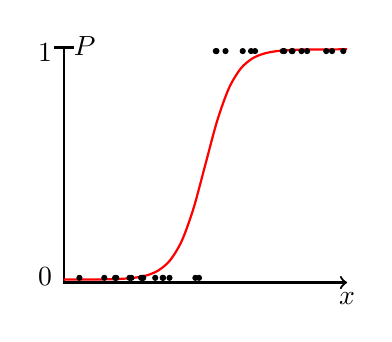
\begin{tikzpicture}[scale=0.15]
	\draw [thick, |->] (-12, 10) node [anchor=west] {\( P \)} -- (-12, -10) -- (12, -10) node [anchor=north] {\( x \)};
	\draw [red, thick, smooth] plot [domain=-12:12] (\x, {(1 / (1 + exp(-0.8*\x)))*19.5 - 9.75});
	\draw plot [only marks, mark=*, mark size=6, domain=-8:8, samples=15] ({12.5*rnd - 0.5}, 9.6);
	\draw plot [only marks, mark=*, mark size=6, domain=-8:8, samples=15] ({-12.5*rnd + 0.5}, -9.6);
	\draw (-15, -9.5) node [anchor=west] {0};
	\draw (-15, 9.5) node [anchor=west] {1};
\end{tikzpicture}

\end{multicols}

\columnbreak

\section*{Incorrect functional form}

\textbf{Ramsey's RESET} (Regression Specification Error Test).

\begin{center}
	\( H_{0} \): The model is correctly specified.
\end{center}

\begin{enumerate}[leftmargin=*]
	\item Estimate the original model and obtain \( \hat{y} \) and \( R^{2} \):
	\begin{center}
		\( \hat{y} = \hat{\beta}_{0} + \hat{\beta}_{1} x_{1} + \cdots + \hat{\beta}_{k} x_{k} \)
	\end{center}
	\item Estimate a model adding powers of \( \hat{y} \) and obtain \( R_{\text{new}}^{2} \):
	\begin{center}
		\( \tilde{y} = \hat{y} + \tilde{\gamma}_{2} \hat{y}^{2} + \cdots + \tilde{\gamma}_{l} \hat{y}^{l} \)
	\end{center}
	\item Test statistic, under \( \gamma_{2} = \cdots = \gamma_{l} = 0 \) as \( H_{0} \):
	\begin{center}
		\( F = \frac{R_{\text{new}}^{2} - R^{2}}{1 - R_{\text{new}}^{2}} \cdot \frac{n - (k + 1) - l}{l} \sim F_{l, n - (k + 1) - l} \)
	\end{center}
\end{enumerate}

If \( F > F_{l, n - (k + 1) - l} \), there is evidence to reject \( H_{0} \).

\section*{Statistical definitions}

Let \( \xi, \eta \) be random variables, \( a, b \in \mathbb{R} \) be constants, and \( P \) denotes probability.

\textbf{Mean} \quad \( E(\xi) = \sum_{i = 1}^{n} \xi_{i} \cdot P[\xi = \xi_{i}] \)

Sample mean: \quad \( \E(\xi) = \dfrac{1}{n} \sum_{i = 1}^{n} \xi_{i} \)

Properties of the mean:

\begin{itemize}[leftmargin=*]
	\item \( \E(a) = a \)
	\item \( \E(\xi + a) = \E(\xi) + a \)
	\item \( \E(a \cdot \xi) = a \cdot \E(\xi) \)
	\item \( \E(\xi \pm \eta) = \E(\xi) + \E(\eta) \)
	\item \( \E(\xi \cdot \eta) = \E(\xi) \cdot \E(\eta) \) \quad only if \( \xi \) and \( \eta \) are independent.
	\item \( \E(\xi - \E(\xi)) = 0 \)
	\item \( \E(a \cdot \xi + b \cdot \eta) = a \cdot \E(\xi) + b \cdot \E(\eta) \)
\end{itemize}

\textbf{Variance} \quad \( \Var(\xi) = \E \left[ (\xi - \E(\xi))^{2} \right] \)

Sample variance: \quad \( \Var(\xi) = \dfrac{\sum_{i = 1}^{n} (\xi_{i} - \E(\xi))^2}{n - 1} \)

Properties of the variance:

\begin{itemize}[leftmargin=*]
	\item \( \Var(a) = 0 \)
	\item \( \Var(\xi + a) = \Var(\xi) \)
	\item \( \Var(a \cdot \xi) = a^{2} \cdot \Var(\xi) \)
	\item \( \Var(\xi \pm \eta) = \Var(\xi) + \Var(\eta) \pm 2 \cdot \Cov(\xi, \eta) \)
	\item \( \Var(a \cdot \xi \pm b \cdot \eta) = a^{2} \cdot \Var(\xi) + b^{2} \cdot \Var(\eta) \pm 2 a b \cdot \Cov(\xi, \eta) \)
\end{itemize}

\textbf{Covariance} \quad \( \Cov(\xi, \eta) = \E \left[ (\xi - E(\xi)) \cdot (\eta - E(\eta)) \right] \)

Sample covariance: \quad \( \dfrac{\sum_{i = 1}^{n} (\xi_{i} - \E(\xi)) \cdot (\eta_{i} - \E(\eta))}{n - 1} \)

Properties of the covariance:

\begin{itemize}[leftmargin=*]
	\item \( \Cov(\xi, a) = 0 \)
	\item \( \Cov(\xi + a, \eta + b) = \Cov(\xi, \eta) \)
	\item \( \Cov(a \cdot \xi, b \cdot \eta) = a b \cdot \Cov(\xi, \eta) \)
	\item \( \Cov(\xi, \xi) = \Var(\xi) \)
	\item \( \Cov(\xi, \eta) = \Cov(\eta, \xi) \)
\end{itemize}

\columnbreak

\section*{Hypothesis testing}

\begin{center}
	\begin{tabular}{ c | c | c }
		                       & \( H_{0} \) true            & \( H_{0} \) false           \\ \hline
		Reject \( H_{0} \)     & False positive              & True positive               \\
		                       & Type I Error \( (\alpha) \) & \( (1 - \beta) \)           \\ \hline
		Not reject \( H_{0} \) & True negative               & False negative              \\
		                       & \( (1 - \alpha) \)          & Type II Error \( (\beta) \)
	\end{tabular}
\end{center}

\columnbreak

Typical one-tail test:

\begin{center}
	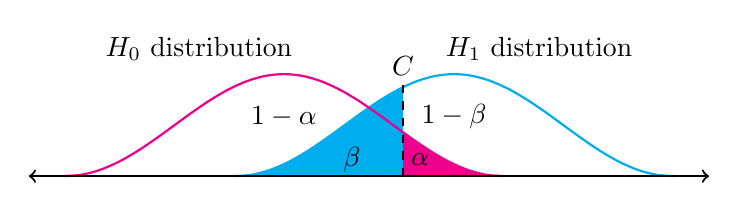
\begin{tikzpicture}[scale=0.108]
		\fill [magenta] (4, 0) -- plot [domain=4:16, smooth] (\x, {cos(\x*7 + 70)*6 + 6}); 
		\fill [cyan] (4, 0) -- plot [domain=-16:4, smooth] (\x, {cos(\x*7 - 70)*6 + 6}); 
		\draw [thick, cyan] plot [domain=-16:36, smooth] (\x, {cos(\x*7 - 70)*6 + 6}); 
		\draw [thick, magenta] plot [domain=-36:16, smooth] (\x, {cos(\x*7 + 70)*6 + 6}); 
		\draw [thick, <->] (-40, 0) -- (40, 0); 
		\draw [thick, dashed] (4, 0) -- (4, 11); 
		\node at (-20, 15) {\( H_{0} \) distribution};
		\node at (20, 15) {\( H_{1} \) distribution}; 
		\node at (-10, 7) {\( 1 - \alpha \)}; 
		\node at (10, 7) {\( 1 - \beta \)}; 
		\node at (6, 2) {\( \alpha \)}; 
		\node at (-2, 2) {\( \beta \)}; 
		\node at (4, 13) {\( C \)};
	\end{tikzpicture}
\end{center}

where \( (1 - \alpha) \) is the confidence level, \( \alpha \) is the significance level, \( C \) is the critical value, \( (1 - \beta) \) is the statistical power.

\section*{Bootstrapping}

\textbf{Problem} - Asymptotic approximations to the distributions of test statistics do not work on small samples.

\textbf{Solution} - Bootstrap is sampling with replacement. The observed data is treated like a population, and multiple samples are extracted to recalculate an estimator or test statistic multiple times (improves accuracy).

\end{multicols}

\begin{multicols}{2}

\section*{VAR (Vector Autoregressive)}

A VAR model captures \textbf{dynamic interactions} between time series. The \( \text{VAR}(p) \):

\begin{center}
	\( y_{t} = A_{1} y_{t - 1} + \cdots + A_{p} y_{t - p} + B x_{t} + CD_{t} + u_{t} \)
\end{center}

where:

\begin{itemize}[leftmargin=*]
	\item \( y_{t} = (y_{1t}, \ldots, y_{Kt})^{\top} \) is a vector of \( K \) observable endogenous time series.
	\item \( A_{i} \)'s are \( K \times K \) coefficient matrices.
	\item \( x_{t} = (x_{1t}, \ldots, x_{Mt})^{\top} \) is a vector of \( M \) observable exogenous time series.
	\item \( B \) is a \( K \times M \) coefficient matrix.
	\item \( D_{t} \) is a vector that contains all deterministic terms: a constant, linear trend, seasonal dummy, and/or any other user-specified dummy variables.
	\item \( C \) is a coefficient matrix of suitable dimension.
	\item \( u_{t} = (u_{1t}, \ldots, u_{Kt})^{\top} \) is a vector of \( K \) white noise series.
\end{itemize}

\textbf{Stability condition}:

\begin{center}
	\( \det(I_{K} - A_{1} z - \cdots - A_{p} z^{p}) \neq 0 \quad \text{for}\quad \lvert z \rvert \leq 1 \)
\end{center}

\quad this is, there are \textbf{no roots} in and on the complex unit circle.

For example, a VAR model with two endogenous variables \( (K = 2) \), two lags \( (p = 2) \), an exogenous contemporaneous variable \( (M = 1) \), a constant \( (\const) \) and a trend \( (\trend) \):

\begin{center}
	\scalebox{0.80}{
		\(
		\begin{bmatrix}
			y_{1t} \\
			y_{2t}
		\end{bmatrix}
		=
		\begin{bmatrix}
			a_{11, 1} & a_{12, 1} \\
			a_{21, 1} & a_{22, 1}
		\end{bmatrix}
		\cdot
		\begin{bmatrix}
			y_{1, t - 1} \\
			y_{2, t - 1}
		\end{bmatrix}
		+
		\begin{bmatrix}
			a_{11, 2} & a_{12, 2} \\
			a_{21, 2} & a_{22, 2}
		\end{bmatrix}
		\cdot
		\begin{bmatrix}
			y_{1, t - 2} \\
			y_{2, t - 2}
		\end{bmatrix}
		+
		\begin{bmatrix}
			b_{11} \\
			b_{21}
		\end{bmatrix}
		\cdot
		\begin{bmatrix}
			x_{t}
		\end{bmatrix}
		+
		\begin{bmatrix}
			c_{11} & c_{12} \\
			c_{21} & c_{22}
		\end{bmatrix}
		\cdot
		\begin{bmatrix}
			\const \\
			\trend
		\end{bmatrix}
		+
		\begin{bmatrix}
			u_{1t} \\
			u_{2t}
		\end{bmatrix}
		\)
	}
\end{center}

Visualizing the separate equations:

\begin{center}
	\( y_{1t} = a_{11, 1} y_{1, t - 1} + a_{12, 1} y_{2, t - 1} + a_{11, 2} y_{1, t - 2} + a_{12, 2} y_{2, t - 2} + b_{11} x_{t} + c_{11} + c_{12} \trend + u_{1t} \)

	\( y_{2t} = a_{21, 1} y_{2, t - 1} + a_{22, 1} y_{1, t - 1} + a_{21, 2} y_{2, t - 2} + a_{22, 2} y_{1, t - 2} + b_{21} x_{t} + c_{21} + c_{22} \trend + u_{2t} \)
\end{center}

If there is a unit root, the determinant is zero for \( z = 1 \); then some or all variables are integrated, and a VAR model is no longer appropriate (it becomes unstable).

\subsection*{SVAR (Structural VAR)}

In a VAR model, causal interpretation is not explicit, and results are sensitive to variable ordering. A SVAR extends VAR by imposing theory-based restrictions on \( \mathsf{A} \) and/or \( \mathsf{B} \) matrices. This can enable causal interpretation and shock analysis without reliance on arbitrary ordering.

For example, a basic \( \text{SVAR}(p) \) model:

\begin{center}
	\( \mathsf{A} y_t = \mathsf{A} [A_1, \ldots, A_p] y_{t - 1} + \mathsf{B} \varepsilon_t \)
\end{center}

where:

\begin{itemize}[leftmargin=*]
	\item \( u_t = \mathsf{A}^{-1} \mathsf{B} \varepsilon_t \)
	\item \( \mathsf{A} \), \( \mathsf{B} \) are \( (K \times K) \) matrices.
\end{itemize}

\columnbreak

\section*{VECM (Vector Error Correction Model)}

If \textbf{cointegrating relations} are present in a system of variables, the VAR form is not the most convenient. It is better to use a VECM, that is, the levels VAR, subtracting \( y_{t - 1} \) from both sides. The \( \text{VECM}(p - 1) \):

\begin{center}
	\( \Delta y_{t} = \Pi y_{t - 1} + \sum_{i = 1}^{p - 1} \Gamma_{i} \Delta y_{t - i} + B x_{t} + CD_{t} + u_{t} \)
\end{center}

where:

\begin{itemize}[leftmargin=*]
	\item \( \Delta y_{t} = (\Delta y_{1t}, \ldots, \Delta y_{Kt})^{\top} \) is a vector of \( K \) observable endogenous time series.
	\item \( \Pi y_{t - 1} \) is the \textbf{long-term} part.
	\begin{itemize}[leftmargin=*, label={\( \diamond \)}]
		\item \( \Pi = - (I_{K} - A_{1} - \cdots - A_{p}) \) for \( i = 1, \ldots, p - 1 \)
		\item \( \Pi = \alpha \beta^{\top} \)
		\item \( \alpha \) is the \textbf{loading matrix} \( (K \times r) \). It represents the speed of adjustment.
		\item \( \beta \) is the \textbf{cointegration matrix} \( (K \times r) \).
		\item \( \beta^{\top} y_{t - 1} \) is the \textbf{cointegrating equation}. It represents the long-run equilibrium.
		\item \( \rk(\Pi) = \rk(\alpha) = \rk(\beta) = r \) is the \textbf{cointegrating rank}.
	\end{itemize}
	\item \( \Gamma_{i} = - (A_{i + 1} + \cdots + A_{p}) \) for \( i = 1, \ldots, p - 1 \) are the \textbf{short-term} parameters.
	\item \( x_{t} \), \( B \), \( C \), \( D_{t} \) and \( u_{t} \) are as in VAR.
\end{itemize}

For example, a VECM with three endogenous variables \( (K = 3) \), two lags \( (p = 2) \) and two cointegrating relations \( (r = 2) \):

\begin{center}
	\( \Delta y_{t} = \Pi y_{t - 1} + \Gamma_{1} \Delta y_{t - 1} + u_{t} \)
\end{center}

\quad where:

\begin{center}
	\scalebox{0.95}{
		\(
		\Pi y_{t - 1} = \alpha \beta^{\top} y_{t - 1} =
		\begin{bmatrix}
			\alpha_{11} & \alpha_{12} \\
			\alpha_{21} & \alpha_{22} \\
			\alpha_{31} & \alpha_{32}
		\end{bmatrix}
		\begin{bmatrix}
			\beta_{11} & \beta_{21} & \beta_{31} \\
			\beta_{12} & \beta_{22} & \beta_{32}
		\end{bmatrix}
		\begin{bmatrix}
			y_{1, t - 1} \\
			y_{2, t - 1} \\
			y_{3, t - 1}
		\end{bmatrix}
		=
		\begin{bmatrix}
			\alpha_{11} ec_{1, t - 1} + \alpha_{12} ec_{2, t - 1} \\
			\alpha_{21} ec_{1, t - 1} + \alpha_{22} ec_{2, t - 1} \\
			\alpha_{31} ec_{1, t - 1} + \alpha_{32} ec_{2, t - 1}
		\end{bmatrix}
		\)
	}
\end{center}

\vspace*{0.2cm}

\begin{center}
	\( ec_{1, t - 1} = \beta_{11} y_{1, t - 1} + \beta_{21} y_{2, t - 1} + \beta_{31} y_{3, t - 1} \)

	\( ec_{2, t - 1} = \beta_{12} y_{1, t - 1} + \beta_{22} y_{2, t - 1} + \beta_{32} y_{3, t - 1} \)
\end{center}

\quad and

\begin{center}
	\scalebox{0.95}{
		\(
		\Gamma_{1} \Delta y_{t - 1} = 
		\begin{bmatrix}
			\gamma_{11} & \gamma_{12} & \gamma_{13} \\
			\gamma_{21} & \gamma_{22} & \gamma_{23} \\
			\gamma_{31} & \gamma_{32} & \gamma_{33}
		\end{bmatrix}
		\begin{bmatrix}
			\Delta y_{1, t - 1} \\
			\Delta y_{2, t - 1} \\
			\Delta y_{3, t - 1}
		\end{bmatrix}
		\quad
		u_t =
		\begin{bmatrix}
			u_{1} \\
			u_{2} \\
			u_{3}
		\end{bmatrix}
		\)
	}
\end{center}

Visualizing the separate equations:

\begin{center}
	\( \Delta y_{1t} = \alpha_{11} ec_{1, t - 1} + \alpha_{12} ec_{2, t - 1}  + \gamma_{11} \Delta y_{1, t - 1} + \gamma_{12} \Delta y_{2, t - 1} + \gamma_{13} \Delta y_{3, t - 1} + u_{1t} \)

	\( \Delta y_{2t} = \alpha_{21} ec_{1, t - 1} + \alpha_{22} ec_{2, t - 1}  + \gamma_{21} \Delta y_{1, t - 1} + \gamma_{22} \Delta y_{2, t - 1} + \gamma_{23} \Delta y_{3, t - 1} + u_{2t} \)

	\( \Delta y_{3t} = \alpha_{31} ec_{1, t - 1} + \alpha_{32} ec_{2, t - 1}  + \gamma_{31} \Delta y_{1, t - 1} + \gamma_{32} \Delta y_{2, t - 1} + \gamma_{33} \Delta y_{3, t - 1} + u_{3t} \)
\end{center}

\end{multicols}

\end{document}